% ==============================================================================
% CHƯƠNG 5: THỰC NGHIỆM MÔ PHỎNG VÀ CÂU HỎI TỰ KIỂM TRA
% ==============================================================================
\chapter{Thực nghiệm mô phỏng và câu hỏi tự kiểm tra}
\label{chap:thuc_nghiem}

Chương này trình bày chi tiết quy trình thiết kế và kết quả thực nghiệm số thực tế cho 5 kịch bản mô phỏng độc lập bằng ngôn ngữ Python (với \texttt{NumPy}, \texttt{Matplotlib}, \texttt{PyWavelets}, cố định \texttt{seed = 42} để đảm bảo khả năng tái lập), cùng hệ thống câu hỏi tự kiểm tra kèm lời giải chi tiết nhằm minh chứng và củng cố toàn diện bản chất toán học của đề tài. Toàn bộ mã nguồn chương trình được đính kèm tại Phụ lục \ref{app:source_code}.

% ==============================================================================
\section{Kịch bản thực nghiệm và phân tích kết quả mô phỏng}
\label{sec:kich_ban_thuc_nghiem}
% ==============================================================================

\subsection{Thí nghiệm 1: Khảo sát chuyển pha theo số phép đo và độ thưa}
\textbf{Mục tiêu:} Xác định ranh giới chuyển pha (\emph{Phase Transition}) \cite{donoho2006compressed} giữa vùng khôi phục thành công 100\% và vùng thất bại khi thay đổi tỷ lệ nén $\delta = m/n$ và độ thưa $k$.

\textbf{Thiết lập tham số và kết quả thực nghiệm:}
\begin{itemize}
    \item Kích thước tín hiệu cố định $n = 128$; số phép đo $m \in \{20, 35, 50, 65, 80, 95\}$; độ thưa $k \in \{4, 8, 12, 16, 20, 24, 28, 32\}$.
    \item Với mỗi cặp $(m, k)$, thực hiện $T = 15$ lần thử nghiệm Monte Carlo độc lập: sinh ma trận Gaussian $A \in \R^{m \times n}$ chuẩn hóa cột, vector $k$-thưa $x^\natural$, giải Basis Pursuit bằng thuật toán ADMM (\texttt{admm\_bp}) và tính thành công khi $\mathrm{RelErr} = \frac{\normtwo{\widehat{x} - x^\natural}}{\max(1, \normtwo{x^\natural})} < 10^{-3}$.
    \item \textbf{Kết quả ghi nhận:} Trên Hình \ref{fig:phase_transition}, đường ranh giới chuyển pha hiện ra rõ nét: chẳng hạn tại $m = 80$ ($\delta = 0{,}625$), thuật toán đạt tỷ lệ thành công $1{,}00$ với mọi $k \le 28$ và giảm xuống $0{,}73$ tại $k = 32$; tại $m = 50$, tỷ lệ đạt $1{,}00$ ở $k \le 8$, $0{,}93$ ở $k = 12$ và giảm về $0{,}20$ ở $k = 20$.
\end{itemize}

\begin{figure}[htbp]
    \centering
    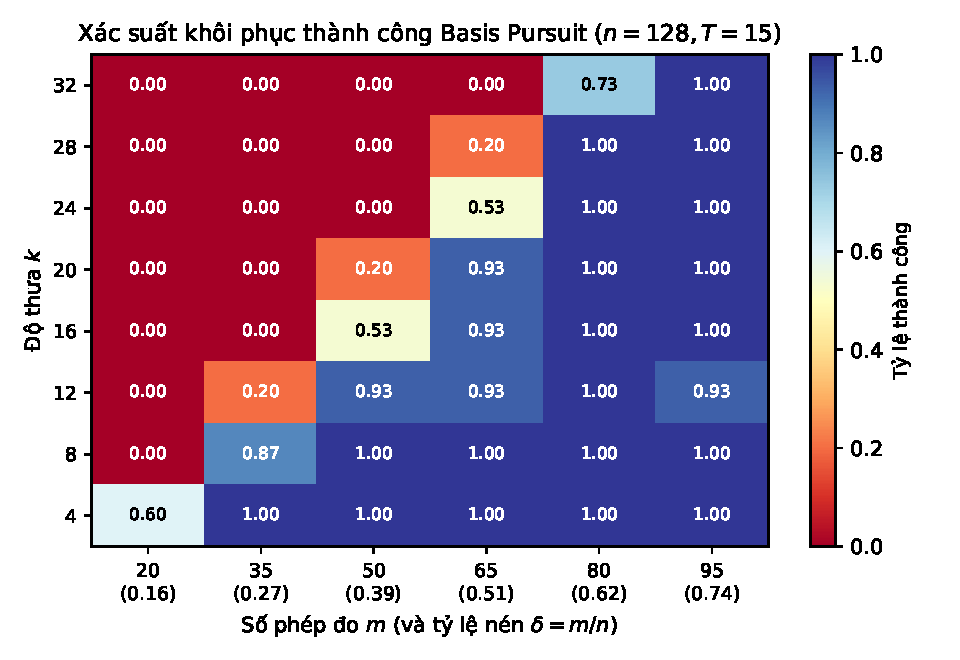
\includegraphics[width=0.82\textwidth]{fig_exp1_phase_transition.pdf}
    \caption{Biểu đồ nhiệt xác suất khôi phục thành công của Basis Pursuit (ADMM) theo $m$ và $k$ ($n = 128, T = 15$, \texttt{seed = 42}).}
    \label{fig:phase_transition}
\end{figure}

\subsection{Thí nghiệm 2: Khảo sát ảnh hưởng của nhiễu và tinh chỉnh tham số $\lambda$}
\textbf{Mục tiêu:} Kiểm chứng chặn sai số ổn định $\|\widehat{x} - x^\natural\|_2 \le C_1 \varepsilon$ và khảo sát đường cong đánh đổi giữa độ khớp dữ liệu và mức độ thưa theo tham số phạt $\lambda$ trong LASSO.

\textbf{Thiết lập tham số và kết quả thực nghiệm:}
\begin{itemize}
    \item Cố định $n = 256, m = 100, k = 12$, nhiễu trắng Gaussian theo 4 mức $\mathrm{SNR} \in \{10, 20, 30, 40\}\text{ dB}$, quét $\lambda$ trên 25 điểm logarit trong $[10^{-4}, 10^0]$ bằng FISTA.
    \item \textbf{Kết quả số thu được:}
    \begin{itemize}
        \item $\mathrm{SNR} = 10\text{ dB}$: $\lambda^* = 2{,}154 \times 10^{-1}$, sai số tương đối nhỏ nhất $\mathrm{RelErr}_{\min} = 0{,}3250$.
        \item $\mathrm{SNR} = 20\text{ dB}$: $\lambda^* = 4{,}642 \times 10^{-2}$, $\mathrm{RelErr}_{\min} = 0{,}1010$.
        \item $\mathrm{SNR} = 30\text{ dB}$: $\lambda^* = 1{,}468 \times 10^{-2}$, $\mathrm{RelErr}_{\min} = 0{,}0314$.
        \item $\mathrm{SNR} = 40\text{ dB}$: $\lambda^* = 4{,}642 \times 10^{-3}$, $\mathrm{RelErr}_{\min} = 0{,}0092$.
    \end{itemize}
    \item Sai số tối ưu giảm theo đúng tỷ lệ $\sqrt{10} \approx 3{,}16$ lần mỗi khi $\mathrm{SNR}$ tăng $10\text{ dB}$, khẳng định tính ổn định tuyến tính theo biên độ nhiễu. Hình \ref{fig:noise_lambda} và Hình \ref{fig:signal_recovery_stem} trình bày kết quả đồ thị thu được.
\end{itemize}

\begin{figure}[htbp]
    \centering
    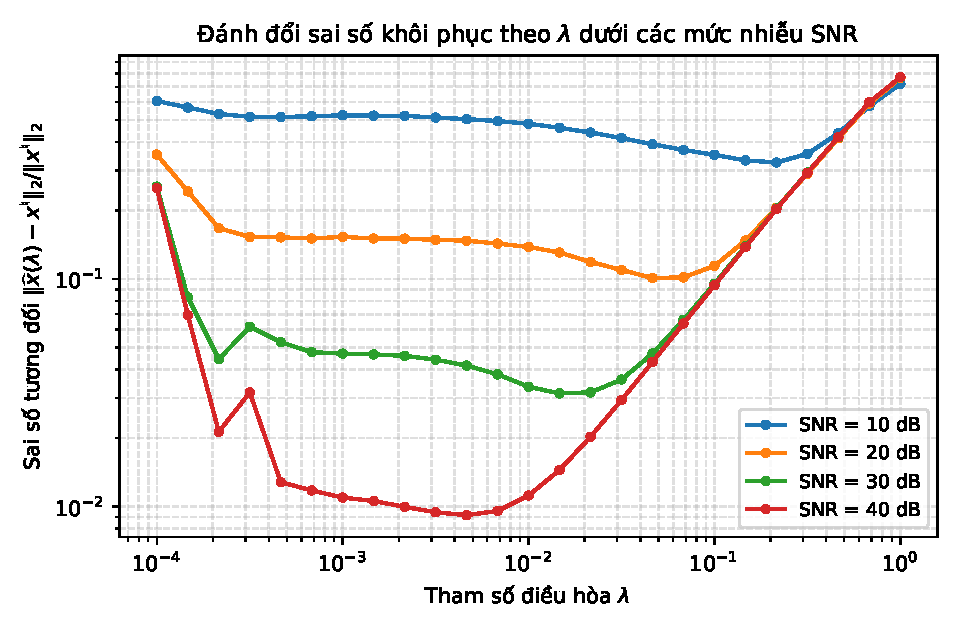
\includegraphics[width=0.80\textwidth]{fig_exp2_noise_lambda.pdf}
    \caption{Đường cong đánh đổi sai số tương đối theo tham số $\lambda$ dưới các mức nhiễu SNR khác nhau.}
    \label{fig:noise_lambda}
\end{figure}

\begin{figure}[htbp]
    \centering
    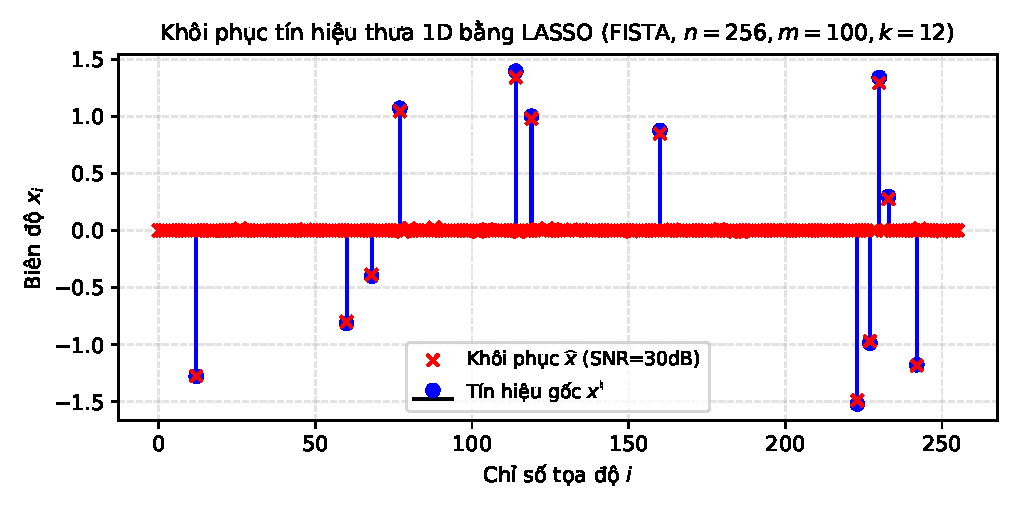
\includegraphics[width=0.86\textwidth]{fig_exp2_stem_1d.pdf}
    \caption{Kết quả khôi phục tín hiệu thưa 1D thực tế tại $\mathrm{SNR} = 30\text{ dB}$ ($n = 256, m = 100, k = 12$): Vị trí và biên độ xung khôi phục $\widehat{x}$ khớp chính xác với tín hiệu gốc $x^\natural$.}
    \label{fig:signal_recovery_stem}
\end{figure}

\subsection{Thí nghiệm 3: So sánh hiệu năng hội tụ giữa ISTA và FISTA}
\textbf{Mục tiêu:} Kiểm chứng bằng thực nghiệm tốc độ hội tụ lý thuyết $\mathcal{O}(1/k)$ của ISTA so với $\mathcal{O}(1/k^2)$ của FISTA.

\textbf{Thiết lập tham số và kết quả thực nghiệm:}
\begin{itemize}
    \item Bài toán LASSO với $n = 512, m = 120, k = 22$, $\sigma = 0{,}01$, $\lambda = 0{,}01 \|A^T b\|_\infty$; hằng số Lipschitz $L$ tính bằng Power Iteration; giá trị tham chiếu $F^* = 0{,}414618$ tính bằng 3.000 vòng lặp FISTA.
    \item \textbf{Kết quả sau 300 vòng lặp:} ISTA đạt $F(x^{300}) - F^* = 6{,}880 \times 10^{-2}$ (thời gian CPU $4{,}25\text{ ms}$), trong khi FISTA đạt $F(x^{300}) - F^* = 2{,}012 \times 10^{-6}$ (thời gian CPU $4{,}79\text{ ms}$) --- cải thiện độ chính xác hơn \textbf{30.000 lần} với chi phí tính toán gần như tương đương (Hình \ref{fig:convergence_comparison}).
\end{itemize}

\begin{figure}[htbp]
    \centering
    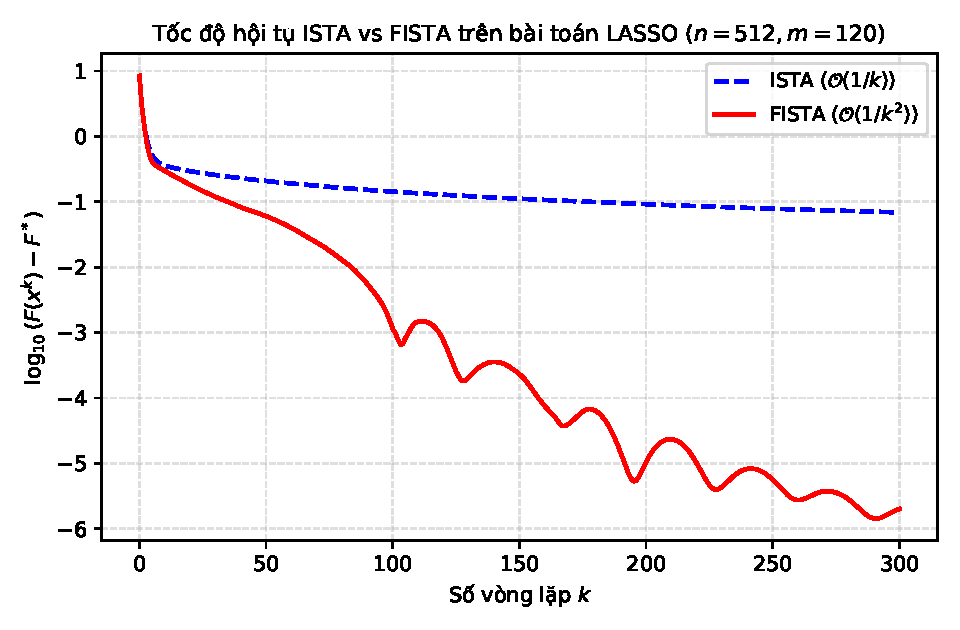
\includegraphics[width=0.80\textwidth]{fig_exp3_ista_vs_fista.pdf}
    \caption{Đồ thị thực nghiệm so sánh tốc độ suy giảm hàm mục tiêu $\log_{10}(F(x^k) - F^*)$ giữa ISTA và FISTA.}
    \label{fig:convergence_comparison}
\end{figure}

\subsection{Thí nghiệm 4: Khảo sát ảnh hưởng của Mutual Coherence}
\textbf{Mục tiêu:} Minh họa kết luận lý thuyết: ma trận có các cột tương quan cao (coherence lớn) sẽ làm suy giảm nghiêm trọng khả năng phục hồi của chuẩn $\ell_1$.

\textbf{Thiết lập tham số và kết quả thực nghiệm:}
\begin{itemize}
    \item Với $m = 80, n = 160, k = 8$ ($T = 25$ lần thử): Ma trận Gaussian độc lập $A$ có $\mu(A) = 0{,}4338$; ma trận $B$ được tạo bằng cách gán cột thứ hai $b_2 = b_1 + \delta$ với $\normtwo{\delta} = 10^{-3}$ rồi chuẩn hóa, cho $\mu(B) \approx 1{,}000000$.
    \item \textbf{Kết quả ghi nhận (Hình \ref{fig:coherence_impact}):} Ma trận $A$ khôi phục thành công $100{,}0\%$. Với ma trận $B$, khi tập hỗ trợ chứa cột $1$ (tương quan cao với cột $2$), tỷ lệ thành công sụt giảm mạnh xuống chỉ còn $16{,}0\%$; ngược lại, khi tập hỗ trợ tránh cặp cột $\{1, 2\}$, tỷ lệ thành công vẫn duy trì $100{,}0\%$.
\end{itemize}

\begin{figure}[htbp]
    \centering
    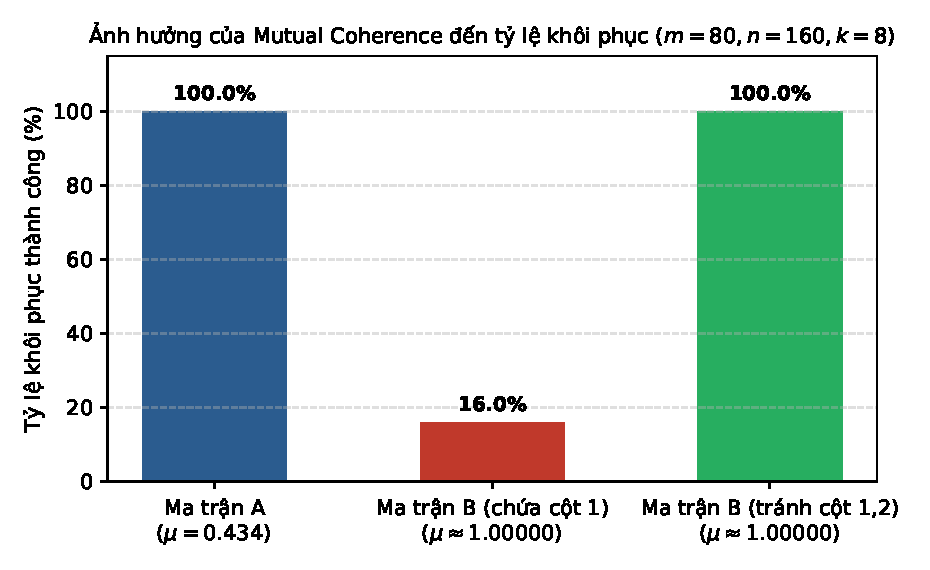
\includegraphics[width=0.78\textwidth]{fig_exp4_coherence.pdf}
    \caption{So sánh tỷ lệ khôi phục thành công của Basis Pursuit trên ma trận coherence thấp ($A$) và ma trận có cặp cột tương quan cao ($B$).}
    \label{fig:coherence_impact}
\end{figure}

\subsection{Thí nghiệm 5: Nén và tái tạo ảnh 2D với biến đổi Wavelet 2D}
\textbf{Mục tiêu:} Đánh giá khả năng ứng dụng thực tiễn của Lấy mẫu nén trên dữ liệu ảnh 2D (thưa xấp xỉ trong miền Wavelet \texttt{db4} mức 3) \cite{nguyen2016khoiphuc}.

\begin{figure}[htbp]
    \centering
    \begin{tikzpicture}[>=stealth, auto, scale=0.92, every node/.style={scale=0.92},
        block/.style={rectangle, draw=blue!80!black, fill=blue!8, thick, rounded corners, minimum height=2.8em, minimum width=5.6em, align=center, font=\footnotesize}]
        
        \node [block] (img) {Ảnh xám gốc\\$x \in \R^{p \times q}$};
        \node [block, right=1.1cm of img] (dwt) {Biến đổi Wavelet 2D\\$\theta = \Psi^T x$ (Thưa)};
        \node [block, right=1.1cm of dwt] (measure) {Đo nén ngẫu nhiên\\$b = A x = A\Psi \theta \in \R^m$};
        
        \node [block, below=1.3cm of measure] (recon) {Thuật toán lồi\\FISTA / ADMM};
        \node [block, left=1.1cm of recon] (idwt) {Wavelet ngược\\$\widehat{x} = \Psi \widehat{\theta}$};
        \node [block, left=1.1cm of idwt] (out) {Ảnh khôi phục\\$\widehat{x}$ ($\mathrm{SSIM} = 0{,}972$)};
        
        \draw [->, thick] (img) -- node [above] {\scriptsize Thưa hóa} (dwt);
        \draw [->, thick] (dwt) -- node [above] {\scriptsize $m \ll n$} (measure);
        \draw [->, thick] (measure) -- node [right] {\scriptsize Dữ liệu $b$} (recon);
        \draw [->, thick] (recon) -- node [above] {\scriptsize Hệ số $\widehat{\theta}$} (idwt);
        \draw [->, thick] (idwt) -- node [above] {\scriptsize Tái tạo ảnh} (out);
    \end{tikzpicture}
    \caption{Sơ đồ khối quy trình nén và tái tạo ảnh xám 2D sử dụng cơ sở biến đổi Wavelet và thuật toán tối ưu hóa lồi.}
    \label{fig:wavelet_cs_pipeline}
\end{figure}

\textbf{Thiết lập tham số và kết quả thực nghiệm:}
\begin{itemize}
    \item Sử dụng ảnh phantom hình học $64 \times 64$ ($n = 4096$ pixel), biến đổi Wavelet Daubechies 4 (\texttt{db4}) mức 3 làm cơ sở $\Psi$, thực hiện $m = 0{,}3n = 1228$ và $m = 0{,}5n = 2048$ phép đo ngẫu nhiên Gaussian và giải bằng 250 vòng lặp FISTA.
    \item \textbf{Kết quả định lượng thực tế (Hình \ref{fig:image_cs_result}):}
    \begin{itemize}
        \item Tại tỷ lệ đo $30\%$ ($m = 0{,}3n$): $\mathrm{PSNR} = 17{,}38\text{ dB}$, $\mathrm{SSIM} = 0{,}869$.
        \item Tại tỷ lệ đo $50\%$ ($m = 0{,}5n$): $\mathrm{PSNR} = 23{,}57\text{ dB}$, $\mathrm{SSIM} = 0{,}972$, tái tạo sắc nét toàn bộ cấu trúc biên và vùng ảnh.
    \end{itemize}
\end{itemize}

\begin{figure}[htbp]
    \centering
    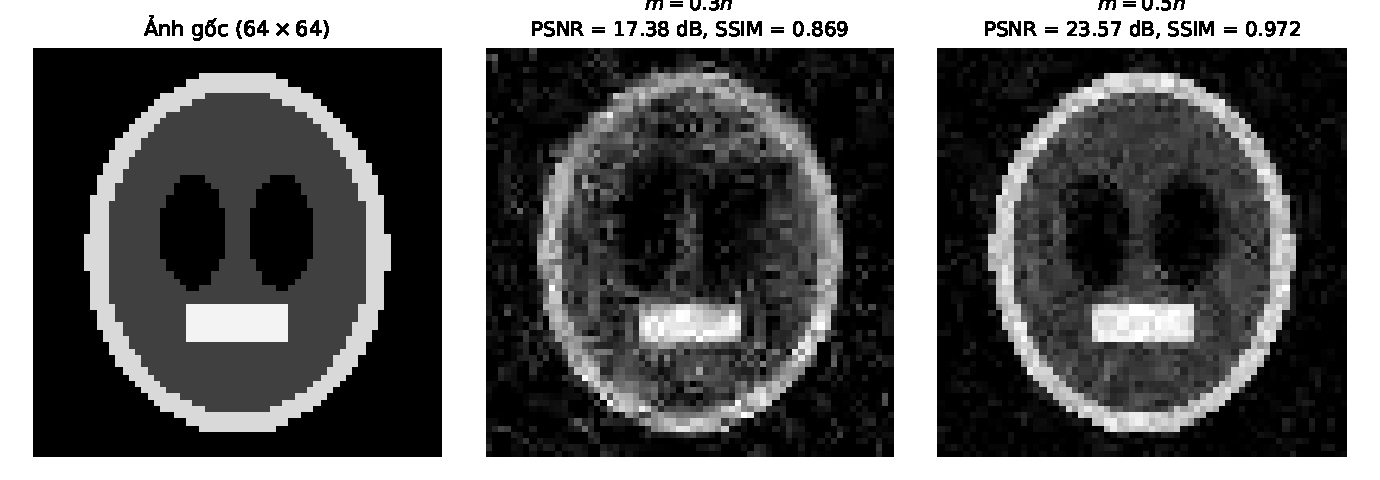
\includegraphics[width=0.95\textwidth]{fig_exp5_image_cs.pdf}
    \caption{Kết quả tái tạo ảnh 2D thực tế bằng FISTA trong miền Wavelet \texttt{db4} tại các tỷ lệ đo $m = 0{,}3n$ và $m = 0{,}5n$.}
    \label{fig:image_cs_result}
\end{figure}

\clearpage

% ==============================================================================
\section{Hệ thống câu hỏi tự kiểm tra và lời giải chi tiết}
\label{sec:cau_hoi_tu_kiem_tra}
% ==============================================================================
Phần này giải quyết trọn vẹn 8 câu hỏi cốt lõi được quy định trong hướng dẫn đề tài, đóng vai trò tự đánh giá mức độ thấu hiểu bản chất toán học từ lý thuyết đến cài đặt thuật toán.

\begin{exercise}[Bài 1: Tính lồi của chuẩn $\ell_1$ và tính không lồi của hàm đếm $\ell_0$]
Chứng minh tính lồi của chuẩn $\normone{x}$ và tính không lồi của đại lượng đếm $\normzero{x}$.
\end{exercise}

\begin{proof}[Lời giải chi tiết]
1. \textbf{Chứng minh chuẩn $\normone{x}$ là hàm lồi trên $\R^n$:}
Theo định nghĩa, hàm $f : \R^n \to \R$ là hàm lồi nếu với mọi $x, y \in \R^n$ và mọi hệ số $\alpha \in [0, 1]$, ta có $f(\alpha x + (1 - \alpha) y) \le \alpha f(x) + (1 - \alpha) f(y)$.
Áp dụng cho chuẩn $\ell_1$:
\[
\normone{\alpha x + (1 - \alpha) y} = \sum_{i=1}^n |\alpha x_i + (1 - \alpha) y_i|.
\]
Với mỗi tọa độ $i \in \{1, \dots, n\}$, sử dụng bất đẳng thức tam giác và tính chất không âm của $\alpha, 1 - \alpha$:
\[
|\alpha x_i + (1 - \alpha) y_i| \le |\alpha x_i| + |(1 - \alpha) y_i| = \alpha |x_i| + (1 - \alpha) |y_i|.
\]
Lấy tổng cả hai vế từ $i = 1$ đến $n$:
\[
\sum_{i=1}^n |\alpha x_i + (1 - \alpha) y_i| \le \alpha \sum_{i=1}^n |x_i| + (1 - \alpha) \sum_{i=1}^n |y_i| = \alpha \normone{x} + (1 - \alpha) \normone{y}.
\]
Điều này chứng minh $\normone{x}$ là hàm lồi trên $\R^n$.

2. \textbf{Chứng minh đại lượng $\normzero{x}$ không phải là hàm lồi:}
Ta chỉ ra một phản ví dụ cụ thể trong $\R^2$. Chọn hai vector $1$-thưa:
\[
x = (2, 0)^T \implies \normzero{x} = 1, \qquad y = (0, 2)^T \implies \normzero{y} = 1.
\]
Lấy hệ số $\alpha = 0.5 \in [0, 1]$, khi đó tổ hợp lồi giữa $x$ và $y$ là:
\[
z = 0.5 x + 0.5 y = (1, 1)^T \implies \normzero{z} = 2.
\]
Trong khi đó, vế phải của bất đẳng thức lồi cho:
\[
\alpha \normzero{x} + (1 - \alpha) \normzero{y} = 0.5(1) + 0.5(1) = 1.
\]
Vì $\normzero{z} = 2 > 1 = \alpha \normzero{x} + (1 - \alpha) \normzero{y}$, bất đẳng thức lồi bị vi phạm. Do đó $\normzero{x}$ không phải là hàm lồi.
\end{proof}

\begin{exercise}[Bài 2: Khôi phục tín hiệu thưa khi số phương trình ít hơn số ẩn ($m < n$)]
Tại sao hệ phương trình tuyến tính $Ax = b$ với $m < n$ vốn có vô số nghiệm lại có thể khôi phục duy nhất tín hiệu ban đầu nếu có thông tin thưa?
\end{exercise}

\begin{proof}[Lời giải chi tiết]
Trong đại số tuyến tính thông thường, nếu $A \in \R^{m \times n}$ với $m < n$, không gian hạt nhân $\ker(A)$ có số chiều ít nhất là $n - m \ge 1$. Do đó, tập nghiệm của hệ $Ax = b$ là một không gian affine $x_0 + \ker(A)$ có vô số phần tử trải dài trên toàn bộ không gian $\R^n$.

Tuy nhiên, tập hợp tất cả các vector $k$-thưa:
\[
\Sigma_k \coloneqq \{x \in \R^n : \normzero{x} \le k\} = \bigcup_{|S| \le k} \{x \in \R^n : \supp(x) \subseteq S\}
\]
không phải là một không gian vector mà là \textbf{hợp của $\binom{n}{k}$ không gian con $k$ chiều}. 
Khi ma trận $A$ thỏa mãn điều kiện cách ly (cụ thể là $\spark(A) > 2k$), không tồn tại bất kỳ vector khác không nào thuộc $\ker(A)$ mà có số tọa độ khác không $\le 2k$. 

Giả sử hệ có hai nghiệm $k$-thưa phân biệt $x, z \in \Sigma_k$ thỏa $Ax = Az = b$. Khi đó hiệu $h = x - z \in \ker(A)$ và thỏa mãn $\normzero{h} = \normzero{x - z} \le \normzero{x} + \normzero{z} \le 2k$. Do $\spark(A) > 2k$, điều này buộc $h = 0 \implies x = z$. 
Như vậy, không gian affine nghiệm $x_0 + \ker(A)$ chỉ cắt tập hợp $\Sigma_k$ tại \textbf{đúng một điểm duy nhất}, loại bỏ hoàn toàn vô số nghiệm không thưa còn lại.
\end{proof}

\begin{exercise}[Bài 3: Phân biệt Spark, NSP và RIP bằng một câu định nghĩa]
Phân biệt sự khác nhau căn bản giữa ba khái niệm trụ cột: Spark, NSP và RIP bằng đúng một câu cho mỗi khái niệm.
\end{exercise}

\begin{proof}[Lời giải chi tiết]
\begin{enumerate}
    \item \textbf{Spark:} Là số lượng cột phụ thuộc tuyến tính nhỏ nhất của ma trận đo $A$, đóng vai trò xác lập điều kiện cần và đủ hình học để nghiệm $k$-thưa là \emph{duy nhất} trong lớp các vector thưa.
    \item \textbf{NSP (Null Space Property):} Là điều kiện phân bố năng lượng chuẩn $\ell_1$ của không gian hạt nhân $\ker(A)$ ra bên ngoài tập hỗ trợ, đóng vai trò là điều kiện cần và đủ để \emph{thuật toán tối ưu lồi Basis Pursuit} tìm ra chính xác nghiệm nguyên bản.
    \item \textbf{RIP (Restricted Isometry Property):} Là tính chất ma trận đo gần như bảo toàn khoảng cách và độ dài Euclid trên tập hợp các vector thưa, đóng vai trò cung cấp công cụ định lượng bảo đảm tính \emph{ổn định bền vững khi phép đo bị ô nhiễm bởi nhiễu}.
\end{enumerate}
\end{proof}

\begin{exercise}[Bài 4: Chứng minh NSP đủ để Basis Pursuit khôi phục chính xác tín hiệu thưa]
Chứng minh tính chất không gian hạt nhân (NSP) bậc $k$ đủ để Basis Pursuit khôi phục đúng mọi vector $k$-thưa.
\end{exercise}

\begin{proof}[Lời giải chi tiết]
Cho $x^\natural \in \R^n$ là vector $k$-thưa tùy ý với tập hỗ trợ $S = \supp(x^\natural)$, thỏa mãn $|S| \le k$ và $x^\natural_{S^c} = 0$. Xét một nghiệm khả thi bất kỳ $x \ne x^\natural$ thỏa mãn hệ phương trình đo $Ax = b$. 
Đặt vector sai số $h \coloneqq x - x^\natural$. Rõ ràng $h \ne 0$ và:
\[
Ah = A(x - x^\natural) = b - b = 0 \implies h \in \ker(A) \setminus \{0\}.
\]
Ta phân tích chuẩn $\ell_1$ của $x = x^\natural + h$ theo hai tập chỉ số rời nhau $S$ và $S^c$:
\[
\normone{x} = \normone{x^\natural_S + h_S} + \normone{x^\natural_{S^c} + h_{S^c}}.
\]
Vì $x^\natural_{S^c} = 0$, ta có:
\[
\normone{x} = \normone{x^\natural_S + h_S} + \normone{h_{S^c}}.
\]
Sử dụng bất đẳng thức tam giác ngược: $\normone{x^\natural_S + h_S} \ge \normone{x^\natural_S} - \normone{h_S}$. Do đó:
\[
\normone{x} \ge \normone{x^\natural_S} - \normone{h_S} + \normone{h_{S^c}} = \normone{x^\natural} + (\normone{h_{S^c}} - \normone{h_S}).
\]
Do ma trận $A$ thỏa mãn tính chất NSP bậc $k$ và $h \in \ker(A) \setminus \{0\}$ với $|S| \le k$, theo định nghĩa NSP ta có $\normone{h_S} < \normone{h_{S^c}}$, dẫn đến:
\[
\normone{h_{S^c}} - \normone{h_S} > 0.
\]
Suy ra:
\[
\normone{x} > \normone{x^\natural}.
\]
Vì mọi nghiệm khả thi $x$ khác $x^\natural$ đều có chuẩn $\ell_1$ thực sự lớn hơn $\normone{x^\natural}$, tín hiệu gốc $x^\natural$ là nghiệm cực tiểu duy nhất của bài toán Basis Pursuit.
\end{proof}

\begin{exercise}[Bài 5: Cơ chế triệt tiêu hệ số $|a_i^T r^*| < \lambda \implies x_i^* = 0$ trong LASSO]
Giải thích tại sao điều kiện tương quan $|a_i^T r^*| < \lambda$ buộc tọa độ thứ $i$ của nghiệm LASSO phải bằng 0 chính xác.
\end{exercise}

\begin{proof}[Lời giải chi tiết]
Bài toán LASSO cực tiểu hóa hàm lồi $F(x) = \frac{1}{2}\normtwo{Ax - b}^2 + \lambda \normone{x}$. 
Điều kiện tối ưu KKT cần và đủ là $0 \in \partial F(x^*)$, tức:
\[
A^T(Ax^* - b) + \lambda \partial \normone{x^*} \ni 0 \iff A^T(b - Ax^*) \in \lambda \partial \normone{x^*}.
\]
Đặt vector phần dư tại nghiệm tối ưu là $r^* = b - Ax^* \in \R^m$. Khi đó $A^T r^* \in \lambda \partial \normone{x^*}$. 
Do chuẩn $\ell_1$ phân tách theo từng tọa độ, xét thành phần thứ $i$:
\[
a_i^T r^* \in \lambda \partial |x_i^*|,
\]
trong đó $a_i$ là cột thứ $i$ của ma trận $A$, và $\partial |x_i^*|$ là dưới vi phân của hàm trị tuyệt đối tại điểm $x_i^*$:
\[
\partial |x_i^*| = 
\begin{cases}
\{\sign(x_i^*)\}, & \text{nếu } x_i^* \ne 0, \\
[-1, 1], & \text{nếu } x_i^* = 0.
\end{cases}
\]
Giả sử phản chứng rằng $x_i^* \ne 0$. Khi đó $\partial |x_i^*| = \{\sign(x_i^*)\}$ với $\sign(x_i^*) \in \{-1, 1\}$, dẫn đến:
\[
a_i^T r^* = \lambda \cdot \sign(x_i^*) \implies |a_i^T r^*| = \lambda |\sign(x_i^*)| = \lambda.
\]
Sử dụng mệnh đề phản đảo: nếu $|a_i^T r^*| \ne \lambda$ (cụ thể là $|a_i^T r^*| < \lambda$), thì giả thiết $x_i^* \ne 0$ không thể xảy ra. Do đó bắt buộc:
\[
x_i^* = 0.
\]
Điều này chứng minh về mặt giải tích rằng tham số $\lambda$ hoạt động như một bộ lọc ngưỡng: chỉ những biến số có mức tương quan giữa cột đo $a_i$ và phần dư $r^*$ đạt đúng giá trị cực đại $\lambda$ mới được phép mang giá trị khác không.
\end{proof}

\begin{exercise}[Bài 6: Chứng minh công thức toán tử co ngưỡng mềm từ dưới vi phân]
Xuất phát từ định nghĩa dưới vi phân bậc nhất, hãy suy ra công thức toán tử co ngưỡng mềm $\mathcal{S}_t(v)$.
\end{exercise}

\begin{proof}[Lời giải chi tiết]
Toán tử co ngưỡng mềm $\mathcal{S}_t(v)$ giải bài toán tối ưu lồi ngặt 1 chiều:
\[
x^* = \argmin_{x \in \R} \phi(x), \quad \text{với } \phi(x) \coloneqq \frac{1}{2} (x - v)^2 + t |x|, \quad (t > 0).
\]
Vì $\phi(x)$ là hàm lồi ngặt liên tục, nghiệm $x^*$ tồn tại và duy nhất, xác định bởi điều kiện Fermat suy rộng:
\[
0 \in \partial \phi(x^*) \iff 0 \in (x^* - v) + t \partial |x^*| \iff v - x^* \in t \partial |x^*|.
\]
Ta xét ba trường hợp của điểm $x^*$:
\begin{enumerate}
    \item \textbf{Trường hợp 1 ($x^* > 0$):} Khi đó $\partial |x^*| = \{1\}$, điều kiện trở thành:
    \[
    v - x^* = t \implies x^* = v - t.
    \]
    Để điều kiện $x^* > 0$ được thỏa mãn, ta cần $v - t > 0 \iff v > t$.
    
    \item \textbf{Trường hợp 2 ($x^* < 0$):} Khi đó $\partial |x^*| = \{-1\}$, điều kiện trở thành:
    \[
    v - x^* = -t \implies x^* = v + t.
    \]
    Để điều kiện $x^* < 0$ được thỏa mãn, ta cần $v + t < 0 \iff v < -t$.
    
    \item \textbf{Trường hợp 3 ($x^* = 0$):} Khi đó $\partial |x^*| = [-1, 1]$, điều kiện trở thành:
    \[
    v - 0 \in t [-1, 1] \iff v \in [-t, t] \iff |v| \le t.
    \]
\end{enumerate}
Hợp nhất cả ba trường hợp lại, ta thu được nghiệm đóng tường minh:
\[
x^* = \mathcal{S}_t(v) = 
\begin{cases}
v - t, & \text{nếu } v > t, \\
0, & \text{nếu } |v| \le t, \\
v + t, & \text{nếu } v < -t,
\end{cases}
= \sign(v) \max(|v| - t, 0).
\]
\end{proof}

\begin{exercise}[Bài 7: Tại sao cần so sánh theo thời gian chạy thực tế thay vì chỉ đếm số vòng lặp?]
Nêu lý do khoa học tại sao khi đánh giá các thuật toán số, việc đo thời gian thực thi (CPU time) lại quan trọng hơn chỉ đếm số lượng vòng lặp.
\end{exercise}

\begin{proof}[Lời giải chi tiết]
Trong phân tích thuật toán tối ưu hóa, chi phí tính toán của một lần lặp phụ thuộc hoàn toàn vào cấu trúc của bài toán con tại mỗi bước:
\begin{itemize}
    \item \textbf{Các thuật toán bậc nhất (ISTA, FISTA):} Mỗi vòng lặp chỉ đòi hỏi hai phép nhân ma trận--vector $Ax$ và $A^T r$ cùng phép co ngưỡng mềm $\mathcal{S}_t(\cdot)$ với chi phí tính toán rất thấp $\mathcal{O}(mn)$.
    \item \textbf{Các phương pháp bậc hai và điểm trong (Interior Point, Newton):} Có tốc độ hội tụ bậc hai tiệm cận và thường hội tụ trong rất ít vòng lặp (chỉ $15 - 30$ vòng lặp). Tuy nhiên, tại mỗi vòng lặp, phương pháp này đòi hỏi phải thiết lập và giải hệ phương trình tuyến tính kích thước $m \times m$ (hệ Newton) hoặc nghịch đảo ma trận, tiêu tốn chi phí $\mathcal{O}(m^3 + m^2n)$ và bộ nhớ khổng lồ.
\end{itemize}
Do đó, nếu chỉ so sánh số vòng lặp, người nghiên cứu sẽ lầm tưởng các thuật toán điểm trong hiệu quả hơn. Trên thực tế với dữ liệu lớn ($n \ge 10^5$), thời gian chạy một vòng lặp điểm trong có thể lâu hơn hàng nghìn vòng lặp của FISTA. Thời gian thực thi CPU phản ánh chân thực chi phí tài nguyên và khả năng mở rộng của thuật toán trong môi trường thực nghiệm.
\end{proof}

\begin{exercise}[Bài 8: Tại sao khi có nhiễu, khôi phục chính xác tuyệt đối không còn là mục tiêu hợp lý?]
Khi dữ liệu đo bị ô nhiễm bởi nhiễu, vì sao mục tiêu khôi phục chính xác tuyệt đối ($\widehat{x} = x^\natural$) không còn khả thi và hợp lý về mặt toán học?
\end{exercise}

\begin{proof}[Lời giải chi tiết]
Xét mô hình đo có nhiễu: $b = A x^\natural + e$ với $e \ne 0$. 
Không gian con sinh bởi $k$ cột tương ứng với tập hỗ trợ thực tế $S = \supp(x^\natural)$ là $\mathcal{R}(A_S) = \{A_S z : z \in \R^k\}$. Vì vector nhiễu $e \in \R^m$ mang tính ngẫu nhiên (ví dụ nhiễu Gaussian), vector quan sát $b = A_S x^\natural_S + e$ hầu như chắc chắn \textbf{không nằm trong không gian con $\mathcal{R}(A_S)$}.

Nếu một thuật toán cố tình ép buộc khôi phục chính xác hệ thức đẳng thức $Ax = b$, thuật toán sẽ buộc phải huy động thêm các cột đo nằm ngoài tập hỗ trợ thực tế ($j \notin S$) để cố gắng khớp phần năng lượng của vector nhiễu $e$. Hiện tượng này gây ra lỗi \textbf{quá khớp nhiễu} (\emph{noise overfitting}), làm sai lệch hoàn toàn tập hỗ trợ và khiến vector khôi phục không còn thưa.

Do đó, mục tiêu toán học đúng đắn khi có nhiễu là \textbf{khôi phục ổn định} (\emph{stable recovery}): chấp nhận sai số tái tạo và kiểm soát sai số này bị chặn tuyến tính theo biên độ năng lượng của nhiễu:
\[
\normtwo{\widehat{x} - x^\natural} \le C_0 \frac{\sigma_k(x^\natural)_1}{\sqrt{k}} + C_1 \normtwo{e}.
\]
Khi biên độ nhiễu tiến về 0 ($\normtwo{e} \to 0$), sai số khôi phục sẽ tiến về 0, bảo đảm tính liên tục và độ bền vững của mô hình.
\end{proof}
